\glspl{MSR} possess unique characteristics which render existing \gls{LWR}
analysis software inappropriate for \gls{MSR} analysis. Legacy \gls{LWR}
software typically scale poorly on modern high-performance computing
clusters and do not support complex geometries beyond regular \gls{LWR} fuel
assembly lattices. Furthermore, \glspl{MSR} feature strong multiphysics
coupling, forcing segregated solvers into taking smaller timesteps to
maintain accuracy. This chapter presents a literature
review of existing multiphysics simulation software developed for \glspl{MSR}
analysis. This work focuses on software for analyzing short-term reactor
dynamics, which requires accurately simulating various transient
scenarios such as reactor start-up and coast-down, load-following operations,
steady-state operation, and accident analysis. Long-term dynamics such as fuel
burnup and structural corrosion fall outside the scope of this work.
This chapter also provides a literature review of turbulence modeling and transport-correction
techniques for the neutron diffusion method relevant to control rod modeling.

\section{MSR Multiphysics Modeling} \label{sec:msr-multiphysics}

The existence of multiple, disparate physics in a single system constitutes a multiphysics system.
Consequently, we need multiphysics software to accurately model a multiphysics system. Employing
well-verified single-physics software for coupled multiphysics simulations does not guarantee
stability, accuracy, or robustness \cite{keyes_multiphysics_2013}. Nevertheless, coupling separate
single-physics software for multiphysics simulations is a viable and popular option with proper
implementation. With strong coupling between different physics, extra care must be
taken to capture various multiphysics interactions accurately. For instance, the two-way coupling
between neutron flux and temperature in \glspl{MSR} described in this section necessitates robust
coupling techniques. Naive multiphysics coupling algorithms may result in longer computation times
at best and non-converging simulations at worst.

Whether one couples separate single-physics software together or develops an
intrinsic multiphysics software, multiphysics software for modeling \glspl{MSR} must employ
\textit{tight coupling schemes} to couple the neutronics
and \gls{TH} governing equations to capture the strong
multiphysics interactions in transient \gls{MSR} simulations accurately. Tightly coupled
numerical models handle multiphysics interactions by either updating all state
variables simultaneously in one monolithic solve (\textit{full coupling}) or
iteratively updating all state variables (\textit{fixed point iterations})
until the solution converges in every timestep \cite{keyes_multiphysics_2013}.
Full coupling tends to be more computationally expensive because it combines
all physics equations into a single large system of equations to be solved
simultaneously. In contrast, fixed point iterations involve operator splitting to
separate the system of equations into smaller systems based on their associated
physics, solving smaller systems separately, and iteratively updating the state
variables until convergence. Fixed point iterative methods are often less
stable, less accurate, and have poorer
convergence rates since these methods make iterative corrections
without regard to potentially destabilizing modes introduced by the
multiphysics coupling \cite{keyes_multiphysics_2013}. In particular, Lindsay et al.
\cite{lindsay_introduction_2018} demonstrated the non-convergence of a multiphysics \gls{MSR}
model when using fixed point iterations. On the other hand, proven
techniques exist for improving the performance of fixed point iteration
coupling schemes for many relevant computational multiphysics research fields,
including reactor analysis \cite{ragusa_consistent_2009}. While fully coupled
schemes solve large systems of equations, they can still outperform
fixed point iterative methods in some multiphysics problems through superior
stability and convergence rates. 

In contrast to tight coupling schemes, \textit{loose coupling schemes}
solve each set of single-physics equations using state variable
data from the previous timestep without iterative corrections within every
timestep. Loosely coupled schemes are inappropriate for modeling \glspl{MSR},
given the strong coupling between neutronics and \gls{TH}.
Aufiero et al. \cite{aufiero_development_2014} demonstrated a loose coupling
approach that failed to reproduce the expected increase in reactor power
in an \gls{MSR} in response to a 150 pcm reactivity insertion.

Consequently, MSR multiphysics simulation tools must employ, at
the very least, tight coupling schemes through fixed-point iterations. The
next subsection reviews existing \gls{MSR} multiphysics simulations and results.

\subsection{Review of MSR Multiphysics Simulations and Results} \label{sec:msr-tools}

Several simulation tools have been developed for \gls{MSR} modeling in the last two decades. Given
the focus on developing high-quality \gls{MSR} software to support reactor design optimization,
this literature review omits MSR simulation work with zero-dimensional point reactor kinetics in
favor of those with spatially-resolved neutronics methods.

Most \gls{MSR} simulation tools employ tight coupling to couple separate neutronics and
\gls{TH} solvers. In 2007, Krepel et al. \cite{krepel_dyn3d-msr_2007} extended the
\gls{LWR} nodal diffusion code DYN3D to account for \gls{DNP} drift and fission energy deposition
in the coolant for \gls{MSR} modeling. The extended DYN3D-MSR code also contains the FLOCAL
\gls{TH} model for coolant flow and conjugate heat transfer modeling. Their \gls{MSRE} and
\gls{MSBR} models consisted of homogeneous hexagonal nodes (mesh elements) for the nodal diffusion
calculation coupled to individual hexagonal unit cells comprising of graphite with circular fuel
channels in the center for the \gls{TH} calculations. They simulated steady-state operation;
start-up, coast-down, natural circulation transients; and an overcooling transient in their
\gls{MSRE} model. They also modeled steady-state operation and a single-channel blockage transient
in their \gls{MSBR} model. At the \gls{TUD}, Kophazi et al. \cite{kophazi_development_2009} coupled
their in-house 3D neutron diffusion software DALTON \cite{boer_validation_2010} and \gls{TH}
software THERM to develop a 3D \gls{MSR} simulation tool. They homogenized the heterogeneous fuel
and graphite region of the \gls{MSRE} for the neutronics calculation. They discretized the
homogeneous region into a Cartesian mesh and modeled a more accurate representation of the oblong
fuel channels in the graphite core matrix instead of the circular shape by Krepel et al.
\cite{krepel_dyn3d-msr_2007}. Both efforts by Krepel et al. and Kophazi et al. showed good
agreement with \gls{MSRE} experimental data in their respective validation tests.
The researchers from \gls{TUD} continued in their approach of coupling separate single-physics
software to create \gls{MSR} simulation tools, as noted by the DALTON-HEAT
\cite{de_zwaan_static_2007} coupling to model the \gls{MSFR} \cite{fiorina_modelling_2014}. The
fast-spectrum \gls{MSFR} features a large pool of fuel salt in its single-channel design instead of
the \gls{MSRE}'s multi-channel design. As a result, the authors had to incorporate
multidimensional turbulent flow modeling to accurately model the complex flow profiles and
turbulence effects in the \gls{MSFR} during steady-state operation and transient scenarios. In a
later effort from the same institute, Tiberga et al. \cite{tiberga_discontinuous_2019} coupled
PHANTOM-$S_N$ and DGFlows in their participation in the CNRS benchmark study
\cite{tiberga_results_2020}. Developed at the \gls{CNRS}, the CNRS benchmark facilitates
code-to-code verification of \gls{MSR} multiphysics software \cite{aufiero_testing_2018}.

Another multiphysics package was developed at
the \gls{PSI} by coupling the \gls{LWR} \gls{TH} system software \gls{TRACE} \cite{nrc_trace_2007}
with the nodal neutron diffusion software \gls{PARCS} \cite{downar_parcs_2010} for safety
analysis of the \gls{MSFR} \cite{pettersen_coupled_2016}. The straight cylinder \gls{MSFR} design
was approximated using hexagonal nodes in \gls{PARCS} while \gls{TRACE} simulated
Reynolds-averaged, inviscid coolant flow. While modeling inviscid flow reduces computational costs
by eliminating the need for expensive turbulence modeling, this approach neglects turbulent flow
and turbulent mixing effects. More recently, Jaradat et al. \cite{jaradat_development_2021}
extended the 3D $P_1$ and $SP_3$ nodal transport code PROTEUS-NODAL to support \gls{DNP} drift.
Yang et al. \cite{yang_development_2022} then developed a coupled simulation tool of PROTEUS-NODAL
and \gls{SAM}. They modeled the \gls{MSFR} on a 2D axisymmetric geometry
and the \gls{MSRE} on a 3D R-$\theta$-Z geometry with twelve 1D flow channels. The \gls{SAM} flow
model relied on the algebraic mixing length model for turbulence modeling. Both results
reproduced the expected trends observed in published experimental and simulation data. Coupling
single-physics software to form integrated multiphysics tools allows researchers to leverage
existing well-validated, single-physics software. These single-physics software are also highly
optimized for solving specific \glspl{PDE} relevant to the investigated system.

With modern advancements in computing hardware and growing access to
high-performance computing systems, others have developed multiphysics tools by
coupling the \gls{CFD} software OpenFOAM
\cite{the_openfoam_foundation_ltd_openfoam_2021} with the Monte Carlo particle
transport software Serpent \cite{leppanen_serpent_2014}, thus achieving
high-fidelity neutronics calculations in transient reactor analyses. To that end,
Serpent has a multiphysics interface supporting coupling
with other physics software \cite{leppanen_development_2013}. Laureau et al.
\cite{laureau_transient_2017} developed a different technique called the
\gls{TFM} method by introducing additional time-dependence
operators to conventional fission matrices typically used to accelerate source
convergence in Monte Carlo neutronics calculations. The \gls{TFM} method
pre-calculates three \glspl{TFM} of the reactor system in Serpent. It
interpolates the matrix values during the actual transient calculations to
incorporate temperature-induced salt expansion and Doppler
effects on the neutron cross sections and, ultimately, the neutron flux. Laureau et al. opted to
subcycle the neutronics calculations by setting smaller timesteps than the \gls{TH} calculations
to take advantage of the differing physics timescales. They demonstrated load-following capability
and parametric studies of overcooling and reactivity insertion transients in the \gls{MSFR}.
Blanco \cite{blanco_neutronic_2020} took a more direct approach by
compiling Serpent as an internal \texttt{C}-based function within OpenFOAM's
\texttt{C++}-based framework. This approach reduced the amount of external data
transfers between Serpent and OpenFOAM as both software have access to shared
memory during runtime. Their integrated tool employs the Quasi-Static
method for transient neutronics calculations and runs Serpent Monte Carlo
calculations several times per timestep until convergence is reached.
Blanco demonstrated the Serpent-OpenFOAM tool on the CNRS benchmark specified by Tiberga et al.
\cite{tiberga_results_2020}.

Another \gls{MSR} simulation approach involves developing inherently multiphysics software that
handle all multiphysics calculations and data transfer internally. Among earlier efforts, Nicolino
et al. \cite{nicolino_coupled_2008} and Zhang et al. \cite{zhang_development_2009} recognized the
need for more robust multiphysics coupling, acceleration techniques and internal data transfers
to reduce execution times. They each independently developed unnamed multiphysics simulation tools
and demonstrated their tools with non-moderated \gls{MSR}
designs. Later, Li et al. \cite{li_transient_2015} demonstrated the
steady-state and transient analysis capabilities of COUPLE, a neutronics and
\gls{TH} software developed at the Karlsruhe Institute of Technology.
Others adopted extensible software frameworks for developing numerical solvers
to develop multiphysics reactor analysis software. Examples of these software
frameworks include the commercial COMSOL
Multiphysics\textsuperscript{\textregistered} software
\cite{comsol_ab_comsol_nodate}, the aforementioned open-source CFD toolbox
OpenFOAM, and the open-source finite-element
framework \gls{MOOSE} \cite{gaston_physics-based_2015}. Researchers at
\gls{PoliMi} developed an \gls{MSR} simulation tool in COMSOL and
modeled the \gls{MSBR} as a single axisymmetric fuel channel with a uniform
flow profile \cite{cammi_multi-physics_2011}, followed by the \gls{MSRE} core
also as a single axisymmetric fuel channel with parabola-shaped laminar flow
\cite{cammi_dimensional_2012}. They later expanded on their approach by
modeling the \gls{MSRE} upper plenum, downcomer and lower plenum, primary heat
exchanger, and secondary heat exchanger as 0D systems (lumped-parameter model)
and substituting the 2D fuel channel with a 3D fuel channel which more closely
resembled the actual fuel channels in the \gls{MSRE}
\cite{zanetti_geometric_2015}. Other than the \gls{MSRE}, they also modeled the
\gls{MSFR} in a later publication \cite{fiorina_modelling_2014}, which also featured \gls{TUD}'s
DALTON-HEAT coupled multiphysics tool.

Other institutes have dedicated significant development work towards
OpenFOAM-based \gls{MSR} simulation tools. Aufiero et al.
\cite{aufiero_development_2014} first introduced an OpenFOAM model developed
at \gls{PoliMi}. Their model implemented a neutron diffusion model and a
\gls{RANS}-based turbulence model under the incompressible flow assumption to demonstrate 2D
and 3D transient analyses of the \gls{MSFR}. Later advancements in the
\gls{PoliMi} solver include a fuel compressibility model with helium bubble
tracking to study fuel compressibility effects
\cite{cervi_development_2019} and an $SP_3$ neutron transport
model for improved neutronics calculations \cite{cervi_development_2019-1} in
the \gls{MSFR}. GeN-Foam is another OpenFOAM-based tool developed by Fiorina
et al. \cite{fiorina_gen-foam_2015} as a general reactor multiphysics solver
applicable to \glspl{MSR} and other reactor types. GeN-Foam features neutron
diffusion, $SP_3$, and $S_N$ neutronics models
\cite{fiorina_development_2016,fiorina_gen-foam_2015,fiorina_detailed_2019},
and thermo-mechanical modeling for reactor expansion effects. Using GeN-Foam,
Altahhan et al. \cite{altahhan_preliminary_2020} developed and optimized a
liquid-fuel \gls{MSR} design, while Shi \& Fratoni \cite{shi_gen-foam_2021}
simulated precursor drift effects in a homogenized \gls{MSRE} model.

Finally, within the \gls{MOOSE} framework, simulation tools capable of modeling
\glspl{MSR} include Griffin \cite{abou-jaoude_coupled_2020}; and Moltres
\cite{lindsay_moltres_2017}\textemdash the subject of this work.
Griffin primarily tackles radiation transport problems, but the \gls{MOOSE}
framework facilitates multiphysics coupling with \gls{MOOSE}-based applications for other physics
such that all applications share the same data structure. This feature eliminates
computational costs from external data transfers and optionally allows for
\textit{fully coupled} calculations in which the application solves all physics
simultaneously. The mutual compatibility among different physics applications within the
\gls{MOOSE} framework simplifies the work required to couple
different physics solvers together to solve novel multiphysics problems. Similarly,
Moltres benefits from the highly-integrated cross-compatibility
within the ecosystem of \gls{MOOSE}-based applications. Abou-Jaoude et al.
\cite{abou-jaoude_coupled_2020} coupled Griffin with Pronghorn, another
\gls{MOOSE}-based application for advanced reactor \gls{TH} modeling, to
demonstrate several steady-state \gls{MSR} simulation capabilities defined in
the CNRS benchmark. Lindsay et al.
\cite{lindsay_introduction_2018} first demonstrated Moltres' \gls{MSR} modeling
capabilities on 2D axisymmetric and 3D Cartesian models of the \gls{MSRE} with
fixed velocity flow on a fully coupled neutronics and \gls{TH} solve.
I later demonstrated some of Moltres' more recent developments through
modeling a 2D axisymmetric model of the \gls{MSFR} for steady-state operation
and transient accident analysis \cite{park_advancement_2020}. The latter study
introduced looped \gls{DNP} flow, coupling the \gls{DNP} drift and temperature 
advection-diffusion to incompressible flow, and decay heat modeling
capabilities.

\subsection{MSR Multiphysics Modeling Verification \& Validation}

\Gls{VV} of simulation models are important components of simulation software development
\cite{sargent_verification_2010}. Verification involves checking whether a model's implementation
accurately represents the conceptual description and specifications. Model
validation is the process of checking whether a model is an accurate representation of the real
world within the range of its intended uses. For reactor software, model verification is commonly
performed by comparing them to other reactor software designed to run the same type of reactor
simulations. On the other hand, model validation is performed by comparing numerical results from
a simulation model to experimental data from the corresponding live test. The validity of a model
depends on the outcome of both model verification and validation.

The important multiphysics phenomena in \glspl{MSR} for model \gls{VV} are salt flow-induced
\gls{DNP} drift and the strong coupling between neutron flux and temperature advection-diffusion.
Delpech et al. \cite{delpech_benchmark_2003}
published one of the first modern \gls{VV} work for \gls{MSR} multiphysics modeling. Collaborators
from six institutions modeled \gls{MSRE} pump start-up, pump coast-down, and natural
circulation transients to assess and validate their models and codes for studying the effects of
salt flow on the reactivity and power. Given the wide range of neutronics methods, from
multidimensional Monte Carlo methods to zero-dimensional point reactor kinetics, some deviations
were observed between different codes. Nevertheless, all results generally agreed
with \gls{MSRE} experimental data from \gls{ORNL}.

As mentioned in Subsection \ref{sec:msr-tools}, Tiberga et al. \cite{tiberga_results_2020}
published the CNRS benchmark to verify \gls{MSR} simulation tools designed for
fast-spectrum \gls{MSR} modeling. In contrast with the multi-channel \gls{MSRE} and its derivative
designs, the CNRS benchmark has a 2 m$\times$2 m problem domain of homogeneous fuel salt mimicking
the large salt pool in fast-spectrum \gls{MSR} designs. The CNRS benchmark consists of three
phases: single-physics calculations in Phase 0, problems that gradually
introduce multiphysics coupling in Phase 1, and time-dependent perturbation problems in Phase
2. Thus, the benchmark provides a systematic approach to help code developers
identify sources of discrepancies that may otherwise be masked by error cancellation or other
dominant sources of discrepancies. The final steady-state and time-dependent problems involve
studying the effects of natural circulation and lid-driven flow on the reactivity and power output.
Aside from the problem specifications, Tiberga et al. also published the associated group
constant cross section data required by deterministic neutronics solvers to perform neutronics
calculations. Four institutions participated in the benchmarking exercise with neutron diffusion,
$SP_N$, and $S_N$-based solvers for the neutronics calculations. Their measured neutronics and
\gls{TH} parameters showed excellent agreement within up to 2.5\% discrepancy from their combined
average.

Neutronic benchmark studies of the \gls{MSRE} and the \gls{MSFR} by Fratoni et al.
\cite{fratoni_molten_2020} and Brovchenko et al. \cite{brovchenko_neutronic_2019} measured the
delayed neutron losses due to the decay of \glspl{DNP} flowing out of the active core region.
Fratoni et al. sought to establish a standard validation platform for \gls{MSR} neutronics
simulation tools with \gls{MSRE} experimental data for inclusion in the \gls{IRPhEP} handbook.
They characterized and validated a model of the \gls{MSRE} in the Monte Carlo particle transport
code Serpent. On the other hand, the \gls{MSFR} benchmark by Brovchenko et al. featured results
from multiple \gls{MSR} simulation tools by several collaborators. Their assessment found that
the choice of nuclear database for the cross sections and decay data has the most significant
impact on the neutronics results.

While these publications have plugged significant technical gaps, there is room to develop further
\gls{VV} benchmarks for multiphysics \gls{MSR} modeling. For instance, the
CNRS benchmark does not assess the loss of delayed neutrons due to the decay of \glspl{DNP} flowing
out of the active core region. This phenomenon is important as the delayed neutron fraction in the
core directly impacts the transient power response in unprotected accident scenarios. Meanwhile,
the neutronic benchmark studies by Fratoni et al. \cite{fratoni_molten_2020} and Brovchenko et al.
\cite{brovchenko_neutronic_2019} did not provide the standardized group constant data required by
most deterministic multiphysics \gls{MSR} simulation tools. Therefore, it is challenging to isolate
discrepancies arising from code implementations instead of discrepancies from using different
nuclear databases or stochastic uncertainties in Monte Carlo simulations. A suitable model
verification procedure for delayed neutron loss should ideally provide well-defined problems and
the necessary input data. It is also helpful to perform model verification studies on simpler
problems like the bare homogeneous problem domain in the CNRS benchmark before embarking on more
detailed validation studies that require accurate models of experimental setups.

\section{Turbulence Modeling in MSRs}

In fluid dynamics, turbulent flow is characterized by unsteady, irregular, and
chaotic fluid motion as opposed to neat, parallel flow layers in laminar flow
\cite{pope_turbulent_2000}. The transition from laminar to turbulent flow
typically occurs at Reynolds numbers between 2000 and 4000, depending on the
setup \cite{pope_turbulent_2000}. Turbulent flows are expected in \glspl{MSR}.
Kedl \cite{kedl_fluid_1970} reports expected Reynolds numbers in the \gls{MSRE}
ranging from 1000 in the regular fuel coolant channels to over 10000 in the
flow distributor volute and core wall cooling annulus regions. For the
\gls{MSFR}, salt flow in the central core region is highly turbulent and
reaches Reynolds numbers on the order of $10^5$.

\subsection{Turbulence Models}

Numerous types of turbulence models exist for various turbulent flow
applications. The most common turbulence models can be classified into the
following categories by order of increasing computational complexity:
%
\begin{itemize}
    \item \gls{RANS}-based models
    \begin{itemize}
        \item Eddy viscosity models
        \begin{itemize}
            \item Algebraic models
            \item One- and two-equation models
        \end{itemize}
        \item \gls{RSM}
    \end{itemize}
    \item \gls{DES}
    \item \gls{LES}
    \item \gls{DNS}
\end{itemize}

\gls{RANS}-based models are based on the \gls{RANS} equations obtained from
applying time-averaging to the fluid flow equations. The \gls{RANS}
equations separate flow into time-averaged $U$ and fluctuating $u$ components
and can be written in Einstein notation and Cartesian coordinates as:
%
\begin{align}
    \frac{\partial U_i}{\partial t} + U_j \frac{\partial u_i}{\partial x_j} =&
    -\frac{1}{\rho} \frac{\partial P}{\partial x_i} + \nu \nabla^2 U_i -
    \frac{\partial \langle u_i u_j \rangle}{x_j}
    \shortintertext{where}
    \langle \cdot \rangle =& \mbox{ time-averaging operator,} \nonumber \\
    \rho =& \mbox{ fluid density,} \nonumber \\
    P =& \mbox{ time-averaged pressure field,} \nonumber \\
    \nu =& \mbox{ kinematic viscosity.} \nonumber
\end{align}

Eddy viscosity models, which comprise the most widely used turbulence models
in use today \cite{rodi_turbulence_2017}, operate on the eddy viscosity
hypothesis which states that the Reynolds stresses in the \gls{RANS} equations
are given by:
%
\begin{align}
    \langle u_iu_j \rangle =& \frac{2}{3}k \delta_{ij} - \nu_T \left(
    \frac{\partial U_i}{\partial x_j} + \frac{\partial U_j}{\partial x_i}
    \right)
    \shortintertext{where}
    k =& \mbox{ mean turbulent kinetic energy,} \nonumber \\
    \delta_{ij} =& \mbox{ Kronecker delta,} \nonumber \\
    \nu_T =& \mbox{ eddy viscosity.} \nonumber \\
\end{align}

The various eddy viscosity models mainly differ in their approach to
the closure problem of calculating the eddy viscosity. As the name suggests,
algebraic models rely on algebraic equations to directly calculate the eddy viscosity
distribution from flow variables. As a result, algebraic models are
the least computationally intensive models for turbulence. Algebraic models
can be further categorized into uniform eddy viscosity models
and mixing length models. Uniform eddy viscosity models apply a uniform eddy
viscosity throughout the problem domain. The uniform eddy viscosity is
calculated from flow parameters such as the characteristic velocity, the
characteristic flow width, and empirically determined turbulent Reynolds
number.

Given that eddy viscosities usually vary significantly in most types of
flow, uniform eddy viscosity models have a limited range of applicability
\cite{pope_turbulent_2000}. Mixing length models add a level of complexity by
relating the eddy viscosity to spatially-varying flow parameters such as the
mean velocity gradient (Prandtl \cite{prandtl_7_1925} and Cebeci-Smith
\cite{smith_numerical_1967} models) or the mean rate of strain (Baldwin-Lomax
\cite{baldwin_thin-layer_1978} model) and an empirical mixing length parameter.
Combined with empirical data for the mixing length parameter, these
models provide better approximations of free shear flows but still
underperform for more complex flows involving flow separation and significant streamline curvature.

One- and two-equation turbulence models introduce differential equations to
describe turbulence quantities such as the turbulence kinetic energy and the
turbulence rate of dissipation to obtain the eddy viscosity distribution. The
most common and best-performing one-equation model is the Spalart-Allmaras
model, which directly provides an equation for the eddy viscosity with several
closure coefficients and functions \cite{wilcox_turbulence_2006}. The
Spalart-Allmaras model is considered ``complete'' as it does not involve
adjustable coefficients or functions. Calibrated for free shear flows in
aeronautical applications, the model performs modestly better than algebraic
models in these applications \cite{pope_turbulent_2000}, but it still deviates
significantly from experimental data
for separated flows \cite{wilcox_turbulence_2006}.

Investigations with
one-equation models reveal the need for an extra equation to account for
turbulent length scales separately from turbulent velocity. Thus, two-equation
models became the most widely adopted turbulence model since the late 20th century
\cite{pope_turbulent_2000}. Two-equation models include the $k$-$\epsilon$,
$k$-$\omega$, and $k$-$\tau$ models. The variables $k$, $\epsilon$, $\omega$,
and $\tau$ correspond to turbulent kinetic energy, turbulent dissipation,
specific turbulent dissipation rate, and turbulent time scale, respectively.
While none of these models perform universally well across all
industrial flows, they are generally more
accurate than the algebraic and one-equation models. Successive contributions
and modifications to the two-equation models through the years have also
improved their performance in predicting various types of turbulent flow. Compared to expensive,
high-fidelity turbulence models, their moderate computational expense favors their adoption in most
commercial \gls{CFD} software for
engineering applications \cite{pope_turbulent_2000}.

\glspl{RSM} directly compute the individual components $\langle u_i u_j
\rangle$ of the Reynolds stress tensor instead of approximating it with a
single, isotropic eddy viscosity term. Consequently, \glspl{RSM} provide
more realistic predictions for flows with significant rotational motion and
sudden changes in the mean strain rate, albeit at greater computational
expense, compared to the one- and two-equation models
\cite{wilcox_turbulence_2006}. More minor improvements are observed in modeling
free shear and backward-facing step flows \cite{wilcox_turbulence_2006}.

Due to the much higher computational cost for \gls{DES}, \gls{LES}, and
\gls{DNS}, these models have limited applicability in routine, high-Reynolds
number engineering problems today. However, given their high accuracy, these
models are useful for flow problems with relatively simple geometries and at
low Reynolds numbers and validating the lower-fidelity turbulence models
\cite{zhiyin_large-eddy_2015}.

\subsection{Turbulence Modeling in MSR Simulation Tools}

Podila et al. \cite{podila_cfd_2019} performed \gls{CFD} simulations of the
\gls{MSRE} core with six different turbulence models, namely a Spalart-Allmaras
model, two variants of the $k$-$\epsilon$ model, a $k$-$\omega$ model, and two
variants of \glspl{RSM}. Their results showed relatively small differences
in graphite and fuel temperatures among different turbulence models. However,
they observed significant differences in the turbulence intensities near the
wall. Given the lack of experimental data for model validation, the authors
could not clearly assess the models' accuracies. Nevertheless, the
close agreement of the fuel temperatures implies that the discrepancies in the
turbulent intensities near the wall have a negligible impact on the overall
distribution of advected quantities in the \gls{MSRE}.

Amongst other \gls{MSR} simulation tools, the $k$-$\epsilon$ and $k$-$\omega$
turbulence models are the most commonly used models, as shown in published work
with COMSOL \cite{fiorina_modelling_2014}, OpenFOAM
\cite{aufiero_development_2014}, and \gls{TUD}'s in-house codes
\cite{fiorina_modelling_2014,tiberga_results_2020}. Fiorina et al.
\cite{fiorina_modelling_2014} compared the flow distribution from both models
in a 2D axisymmetric \gls{MSFR} geometry. They observed that the $k$-$\omega$
model produced a more expansive recirculation zone near the outer wall, an additional
recirculation zone near the top wall, and significantly higher maximum
temperatures within the former recirculation zone.

In a recent study by
Laureau et al. \cite{laureau_unmoderated_2022}, the authors applied a \gls{DES} model to model
eddies in the \gls{MSFR}. Given the high computational costs required to obtain reasonably small
stochastic uncertainties from Monte Carlo calculations on arbitrarily varying temperature fields,
they created a reduced-order model relating local reactivity feedback estimates to the nominal
temperature field to obtain the effective temperature field.
Additionally, they fixed the total
reactor power output to 3 GW to further reduce costs. With this multiphysics model, they found
that the pre-existing \gls{MSFR} model was prone to large power fluctuations of up to 7.5\% under
steady-state operation. Previous studies with lower-fidelity models, including the two-equation
models, failed to capture this effect due to the time-averaging assumption required in those
models. After replacing the large inlet pipes with multiple blade-like inlet channels in the
\gls{MSFR} model, they managed to reduce power fluctuations to 1.2\%.

In essence, the existing literature on turbulence flows in \glspl{MSR} highlight
the importance of modeling turbulent flows and calls for extra care towards the choice of
turbulence model depending on the \glspl{MSR} design and the phenomenon being studied.

\section{Control Rod Modeling in MSRs}

\subsection{Control Rods in MSRs}

The number and locations of control rods in a reactor vary significantly for different reactor
types, depending on their size, refueling frequency, reactivity control systems, and other factors.
\glspl{MSR} contain comparatively fewer control rods than most other reactor types due to the
stability and reactivity control capability provided by the large negative temperature
reactivity feedback. For instance, the \gls{MSRE} contained three rods, while the \gls{MSBR}
developers recommended two to four rods for the \gls{MSBR} \cite{robertson_msre_1965,
robertson_conceptual_1971}. The
strong temperature feedback allows operators to control reactivity by varying salt pump
speeds or heat removal rates. Many \gls{MSR} designs include control rods to facilitate reactor
start-up or shut-down rather than reactivity control during power operation. Using
control rods to achieve even fuel burnup is not a concern for \glspl{MSR} due to the liquid fuel
form. Nevertheless, it is important to characterize control rod effects in all scenarios which
involve the rods.

There is a lack of research into improving control rod modeling in \glspl{MSR}.
The self-regulating nature and low excess reactivity of \glspl{MSR} reduce or even eliminate the
need for control rods \cite{dolan_1_2017}. This characteristic arises from the strongly negative
temperature reactivity feedback and the strong coupling to flow and heat removal rates. \gls{MSR}
reactor designers rely on these passive mechanisms for reactor safety. In addition, they propose
load-following operation by adjusting pump speeds and the temperature of the intermediate coolant
loop. Laureau et al. \cite{laureau_transient_2017} demonstrated simple power ramp-up and ramp-down
with the \gls{MSFR} by varying the temperature of the secondary coolant. \gls{MSR}
designs with no control rods include the fast-spectrum \gls{MSFR} and TerraPower's \gls{MCFR}
\cite{terrapower_terrapower_2021}. However, \gls{MSR} power control schemes which rely heavily on
these mechanisms may not be suitable for all accident scenarios. Control rod insertion can provide
an additional means of reactor shut-down without draining the fuel salt and
complicating reactor restart procedures. We also note that thermal \gls{MSR} designs like the
\gls{MSRE}, \gls{MSBR}, and TMSR-LF1 designs still include control rods as essential components,
partly due to their less negative temperature reactivity feedback coefficients
compared to their fast-spectrum counterparts. Thus, the existing literature on control rod modeling
in \glspl{MSR} are based on thermal-spectrum \glspl{MSR}.

Few \gls{MSR} multiphysics studies explicitly include control rods in their models. For instance,
for the \gls{MSRE} pump start-up and coast-down experiments at \gls{ORNL} which involved control
rod movement, most numerical studies simulate the reactivity effects of the control rods by scaling
the neutron source term by the neutron multiplication factor to keep their reactor model at
criticality \cite{delpech_benchmark_2003, krepel_dyn3d-msr_2007}. Some studies include control rod
models in their steady-state calculations. However, they resort to neutron source term scaling for
the transient calculations due to the inaccuracy of neutron diffusion, $P_1$, and $SP_N$ methods in
highly neutron absorbing regions \cite{kophazi_development_2009, jaradat_development_2021,
yang_development_2022}. Kophazi et al. \cite{kophazi_development_2009} modeled annular control rods
as homogenized hexahedrons in their 3D Cartesian geometry of the \gls{MSRE}. They
homogenized fuel and graphite regions in the rest of the reactor model, as mentioned in Subsection
\ref{sec:msr-tools}. To reduce errors introduced by the neutron diffusion method, they imposed
simple albedo boundary conditions for the thermal neutron group. Jaradat et al.
\cite{jaradat_development_2021} and Yang et al. \cite{yang_development_2022} modeled the \gls{MSRE}
control rods as homogenized wedges in their R-$\theta$-Z mesh due to the constraints of the nodal
neutronics solver. Cui et al. \cite{cui_development_2021} also homogenized the control rods as
regular hexahedral nodes in accordance with their nodal solver in Cartesian geometry. A disadvantage
of homogenization-based methods is that it removes some of the heterogeneity in the flux and
temperature. The heterogeneous temperature distribution is especially important in \glspl{MSR} due
to the combined fuel-coolant and the positive temperature reactivity feedback observed
in graphite under certain conditions \cite{mathieu_thorium_2006}.

In theory, multiphysics simulation tools with Monte Carlo neutron transport, such as the
Serpent-OpenFOAM tool developed by Blanco \cite{blanco_neutronic_2020} could boast excellent
control rod modeling performance. However, the computational cost would be extremely high for
reactor geometries much more complex than the 2 m$\times$2 m homogeneous domain of the CNRS
benchmark (Subsection \ref{sec:msr-tools}). Other high-fidelity neutronics methods, such as the
$S_N$ and $P_N$ methods are also typically too computationally expensive for time-dependent
multiphysics simulations. On the other hand, less taxing methods, such as the neutron diffusion
method, cannot model control rods accurately. The remainder of this section describes the
challenges of control rod modeling with neutron diffusion and reviews existing transport
correction techniques for improving neutron diffusion method performance in control rod modeling.

\subsection{Summary of Neutronics Methods} \label{sec:summary-nts-mtds}

High-fidelity neutron transport methods fall under two general categories: stochastic Monte Carlo
methods and deterministic methods. Monte Carlo methods involve simulating a finite number of
neutron histories. Randomly generated numbers determine the outcome of various probabilistic events
such as travel distances between particle collisions, types of collisions, and scattering angles in
each history until a neutron capture event terminates it. Deterministic methods for neutron
transport, such as the discrete ordinates $S_N$ and spherical harmonics $P_N$ methods, solve the
\gls{BTE} for neutron transport with some approximations for handling the angular and energy
dependence. The \gls{BTE} for neutron transport is given as:
%
\begin{align}
  \frac{1}{v(E)} \frac{\partial}{\partial t} \Psi(\vec{r},E,\hat{\Omega},&t) + \hat{\Omega}\cdot
  \nabla\Psi(\vec{r},E,\hat{\Omega},t) + \Sigma_t(\vec{r},E,t)\Psi(\vec{r},E,\hat{\Omega},t) 
  \nonumber \\
  - \int^\infty_0 dE'& \int_{4\pi} d\hat{\Omega}' \Sigma_s(\vec{r},E'\rightarrow E,\hat{\Omega}'
  \rightarrow \hat{\Omega},t) \Psi(\vec{r},E',\hat{\Omega}',t) \nonumber \\
  =& \frac{\chi(E)}{4\pi}
  \int^\infty_0 dE' \int_{4\pi} d\hat{\Omega}' \nu\Sigma_f(\vec{r},E',t) \Psi(\vec{r},E',
  \hat{\Omega}',t)+S(\vec{r},E,\hat{\Omega}',t) \label{eq:bte}
  \shortintertext{where}
  v(E) =& \mbox{ neutron velocity,} \nonumber \\
  \Psi(\vec{r},E,\hat{\Omega},t) =& \mbox{ neutron angular flux,} \nonumber \\
  \vec{r} =& \mbox{ spatial coordinates,} \nonumber \\
  E =& \mbox{ neutron energy,} \nonumber \\
  \hat{\Omega} =& \mbox{ direction of neutron travel,} \nonumber \\
  t =& \mbox{ time,} \nonumber \\
  \Sigma_t(\vec{r},E,t) =& \mbox{ macroscopic total cross section,} \nonumber \\
  \Sigma_s(\vec{r},E'\rightarrow E,\hat{\Omega}'\rightarrow \hat{\Omega},t) =&
  \mbox{ macroscopic scattering cross section,} \nonumber \\
  \chi(E) =& \mbox{ fission neutron spectrum,} \nonumber \\
  \nu =& \mbox{ number of neutrons produced per fission reaction,} \nonumber \\
  \Sigma_f(\vec{r},E',t) =& \mbox{ macroscopic fission cross section,} \nonumber \\
  S(\vec{r},E,\hat{\Omega}',t) =& \mbox{ external neutron source.} \nonumber
\end{align}

The $S_N$ method discretizes the continuous angular directional phase space into a few discrete
angular directions (ordinates). It uses quadrature rules to replace the integrals over
$\hat{\Omega}$ with summations over the ordinates. On the other hand, the $P_N$ method introduces
Legendre polynomial expansions of the angular flux to approximate the angular dependence. Both
methods require higher-order approximations to produce more accurate flux solutions through more
discrete ordinates or higher-order Legendre expansions. Both methods also discretize the
continuous energy dependence into discrete neutron energy groups, which cover non-overlapping,
finite energy ranges across the entire energy spectrum to form multigroup equations as follows:
%
\begin{align}
  \frac{1}{v_g} \frac{\partial}{\partial t} \Psi_g(\vec{r},\hat{\Omega},&t) + \hat{\Omega}\cdot
  \nabla\Psi_g(\vec{r},\hat{\Omega},t) + \Sigma_{t,g}(\vec{r},t)\Psi_g(\vec{r},\hat{\Omega},t)
  \nonumber \\
  - \sum^G_{g'=1}& \int_{4\pi} d\hat{\Omega}' \Sigma_s^{g'\rightarrow g}(\vec{r},\hat{\Omega}'
  \rightarrow \hat{\Omega},t) \Psi_{g'}(\vec{r},\hat{\Omega}',t) \nonumber \\
  =& \frac{\chi_g}{4\pi}
  \sum^G_{g'=1} \int_{4\pi} d\hat{\Omega}' \nu\Sigma_{f,g'}(\vec{r},t) \Psi_{g'}(\vec{r},
  \hat{\Omega}',t)+S_g(\vec{r},\hat{\Omega}',t) \label{eq:mg-bte}
  \shortintertext{where}
  G =& \mbox{ total number of energy groups,} \nonumber \\
  g =& \mbox{ neutron energy group index (in decreasing energy order)} = 1,2,...,G. \nonumber
\end{align}

The subscript $g$ denotes the corresponding quantity for neutrons in energy group $g$.
Neutron transport methods are very computationally expensive and, thus, are mainly used for
time-independent neutronic analyses. For time-dependent multiphysics simulations coupling
neutronics to \gls{TH} and other physics present in nuclear reactors, most reactor codes
rely on the neutron diffusion equation for modeling neutronics. The multigroup neutron diffusion
equations are \glspl{PDE} derived from Eq. \ref{eq:mg-bte} by making
simplifying assumptions on the angular dependence in the scattering cross section and integrating
the equations over all solid angles to eliminate angular dependence as follows:
%
\begin{align}
  \frac{1}{v_g} \frac{\partial}{\partial t} \phi_g&(\vec{r},t) + \nabla\cdot J_g(\vec{r},t)
  +\Sigma_{t,g}(\vec{r},t) \phi_g(\vec{r},t) \nonumber \\
  =& \sum^G_{g'=1}\left[\Sigma_s^{g'\rightarrow g}
  \phi_{g'}(\vec{r},t) + \chi_g \nu\Sigma_{f,g'} \phi_{g'}(\vec{r},t)\right] + S_g(\vec{r},t)
  \label{eq:mg-diff} \\
  \shortintertext{where}
  J_g(\vec{r},t) =& \mbox{ neutron current for neutron group $g$.} \nonumber
\end{align}

Fick's first law of diffusion provides a closure relation for Eq. \ref{eq:mg-diff} by relating the
current to the flux:
%
\begin{align}
  J_g(\vec{r},t) =& -D_g(\vec{r},t)\nabla\phi_g(\vec{r},t) \label{eq:fick}
  \shortintertext{where}
  D_g(\vec{r},t) =& \mbox{ neutron diffusion coefficient for neutron group $g$.} \nonumber
\end{align}

The diffusion coefficient itself is estimated from the total or transport cross sections, depending
on whether we take scattering to be isotropic or linearly anisotropic in the $P_1$ approximation of
the \gls{BTE} \cite{lamarsh_introduction_1975}:
%
\begin{align}
  D(\vec{r},t) =& \frac{1}{3\Sigma_t(\vec{r},t)} \quad \mbox{(isotropic)} \\
  D(\vec{r},t) =& \frac{1}{3\Sigma_{tr}(\vec{r},t)} = \frac{1}{3\left(\Sigma_t(\vec{r},t)-
  \bar{\mu}\Sigma_s(\vec{r},t)\right)}
  \quad \mbox{(linearly anisotropic)} \label{eq:p1-diffcoef}
  \shortintertext{where}
  \Sigma_{tr} =& \mbox{ macroscopic transport cross section,} \nonumber \\
  \bar{\mu} =& \mbox{ average cosine of the scattering angles.} \nonumber
\end{align}

This treatment significantly reduces the number of coupled \glspl{PDE} to be solved and the
computational costs of modeling neutronics in reactors. However, the simplifications limit the
validity of the neutron diffusion equation to regions of high scattering-to-absorption ratios at
least a few mean free paths away from shared interfaces to neighboring media with highly dissimilar
neutronic properties \cite{shultis_chapter_2016}. Neutron diffusion theory cannot capture the
strongly anisotropic flux within and near control rod regions.

Many legacy diffusion solvers are based on coarse-mesh or nodal methods. These methods
primarily involve replacing heterogeneous lattices of materials of differing properties with
equivalent homogeneous mixtures of the same materials in each coarse mesh (referred to as nodes in
nodal methods) \cite{stacey_nuclear_2007}. Reducing the heterogeneity of the geometry reduces
computational complexity and circumvents poor diffusion performance in highly heterogeneous
interfaces. Each coarse mesh typically corresponds to a subregion comprising of repeating
substructures, e.g. a single fuel assembly or randomly distributed spherical fuel pebbles. The
homogenization procedure consists of two main steps: a transport calculation to obtain detailed
heterogeneous flux distribution within each subregion, and the calculation of homogenized
\textit{group constants} from the detailed flux distribution. \textit{Group constants} refer to
macroscopic neutron cross section values for various neutron interactions such as
scattering, absorption, and fission. Macroscopic cross sections represent the probability that a
neutron, in a given energy range, will undergo the associated interaction per unit distance
traveled in the material. Group constants also broadly include neutron diffusion
coefficients/constants and \gls{DNP} data. While advanced coarse-mesh and nodal
methods provide reasonable flux solutions for calculating global and intermediate-scale quantities,
they do not capture detailed heterogeneous flux distribution within each coarse-mesh subregion.

\subsection{Transport-Correction Techniques With Neutron Diffusion-Based Solvers}

Transport-correction techniques for diffusion-based solvers require additional information beyond
conventional homogenized group constants from transport-based solvers to ameliorate diffusion
solution accuracy in highly absorbing and near-interface regions.
Therefore, this literature review focuses on hybrid diffusion-transport methods developed to relay
transport-corrections to diffusion-based solvers for more accurate neutron flux and current
estimates. The hybrid methods differ mainly in how they incorporate corrections into a
diffusion-based solver. While this work focuses on improving diffusion-based control rod
modeling in Moltres for \gls{MSR}-like designs, this literature review explores existing methods
developed for other reactor types, as no advanced techniques have been applied to \glspl{MSR}.

\subsubsection{Absorber Blackness and Linear Extrapolation Length}

Methods based on absorber blackness \cite{davison_influence_1951, spinks_extrapolation_1965,
pellaud_extrapolation_1968, mendelson_two-dimensional_1969} encompass a
broad class of procedures for generating boundary conditions to match approximate solutions of
low-order methods (e.g., diffusion) to more accurate solutions from high-order methods (e.g.,
transport). The internal boundary conditions replace absorber regions and mimic their presence in
the problem domain. The boundary conditions are generalizations of the Marshak boundary condition
\cite{marshak_note_1947}, which in 1D are of the form:
%
\begin{align}
  \frac{\phi(x)}{d\phi(x)/dx} =& \lambda \label{eq:marshak}
  \shortintertext{where}
  \lambda =& \mbox{ linear extrapolation length.} \nonumber
\end{align}
%
The flux gradient in the denominator is taken in the outward direction at the surface of the
absorber or black body. In Cartesian coordinates, it is common to approximate Eq. \ref{eq:marshak}
in the form:
%
\begin{align}
  \phi(x+\lambda) =& 0
\end{align}
because Dirichlet boundary conditions are easier to work with analytically and numerically.
The corresponding relations in cylindrical and spherical coordinates depend on the radius of the
absorber rod. Various forms for $\lambda$ exist for specific absorber geometries such as slabs
\cite{maynard_blackness_1959} and cylinders \cite{spinks_extrapolation_1965,
pellaud_extrapolation_1968} which were dependent
on the size of the absorber region and coefficients quantifying the escape probability of neutrons
entering the absorber region. The $\lambda$ and the associated coefficients were derived
analytically from the \gls{BTE} with some simplifying assumptions, such as having uniform or
cosine-shaped incident neutron currents, isotropic scattering within the absorber, and mathematical
approximations in ignoring higher-order terms in intermediate steps. Blackness theory emerged in
the mid-20th century when computational resources were limited. Later, as computational
resources became more readily available and powerful enough for more complicated transport
calculations, appropriate boundary conditions could be calculated numerically
\cite{bretscher_computing_1997}. Alternatively, effective group constants can be calculated for
diffusion codes not programmed to handle internal boundary conditions. For instance,
Bretscher \cite{bretscher_computing_1997} provided formulae for effective diffusion coefficient and
absorption cross section for thin absorber slabs as a function of blackness coefficients, absorber
thickness, and mesh size.

Diffusion calculations with corrections from blackness theory can generally provide control rod
worths that reasonably agree with more accurate transport calculations. However, the
diffusion flux distributions still deviate significantly from transport calculations because no
corrections are introduced in the adjacent regions near the absorber where the angular flux can be
strongly anisotropic.

\subsubsection{Method of Equivalent Cross Sections}

Scherer \& Neef developed the \gls{MECS} \cite{scherer_determination_1976} to improve control rod
modeling in \gls{HTGR} with mesh-centered nodal diffusion methods. The \gls{MECS} involves running
a 1D neutron transport calculation on a representative \textit{supercell} of the heterogeneous
absorber region and its vicinity. The supercell is a volume-preserved model of the absorber region
approximated from its cylindrical or Cartesian geometry in the diffusion calculation. The transport
calculation is typically performed using a fine group structure, fine spatial discretization, and
high-order angular discretization and scattering moments (e.g., $S_8$ method with $P_3$ scattering
matrix) \cite{fen_modelling_1992}. The calculated net neutron leakage rates from the transport
solver are matched with the calculated leakage rates from the diffusion solver according to an
analytic calculation to obtain equivalent diffusion coefficients or cross sections for the absorber
region. The diffusion coefficient formula for this analytic calculation depends on the solution
method of the diffusion solver. In the most widely used implementation of \gls{MECS} used in
conjunction with the mesh-centered diffusion code CITATION \cite{teuchert_vsop94_1994}, the
diffusion coefficient formula assumes there is only one inner mesh point in the absorber region as
using more inner mesh points dramatically increases the difficulty of finding the proper analytic
formula \cite{fen_modelling_1992}. Other macroscopic cross sections for the absorber region are
calculated using conventional group constant generation techniques from the transport solution
using the supercell average flux and reaction rates. To facilitate further discussion of the
\gls{MECS}, here is an example of applying the \gls{MECS} on a control rod in x-y geometry (Figure
\ref{fig:mecs-geometry}) in the CITATION code as provided by Fen et al. \cite{fen_modelling_1992}.
%
\begin{figure}[htb]
    \centering
    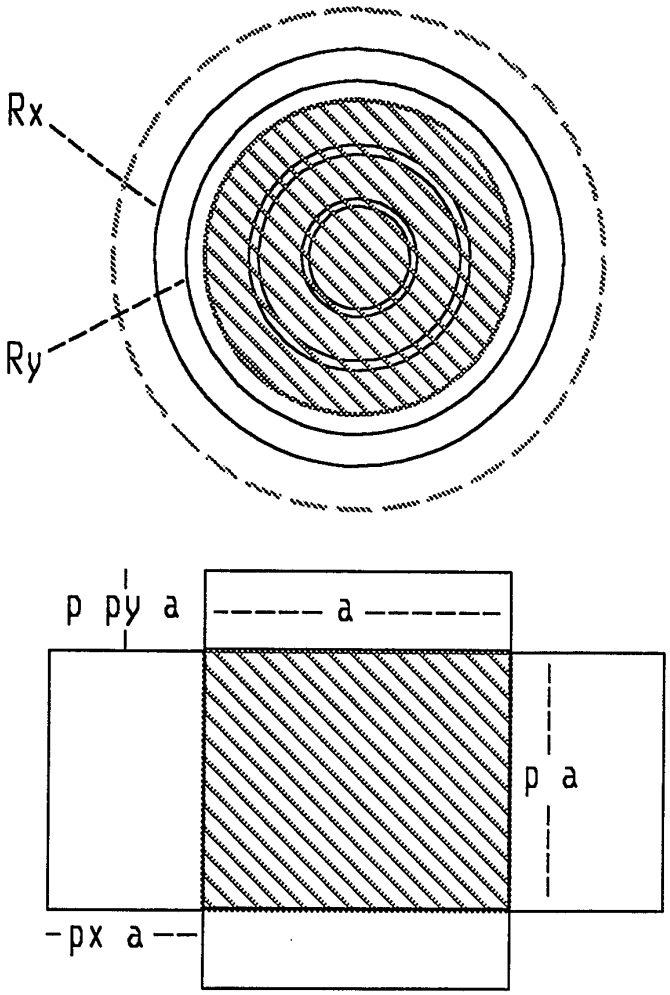
\includegraphics[width=.4\columnwidth]{mecs-geometry}
    \caption{Geometries of the absorber region and its vicinity in the supercell
      (top) and the diffusion solver mesh (bottom).
        The shaded and unshaded regions represent the homogenized absorber
        region and the adjacent non-absorber region, respectively.
        Retrieved from Fen et al. \cite{fen_modelling_1992}.}
    \label{fig:mecs-geometry}
\end{figure}

Figure \ref{fig:mecs-geometry} shows the 1D cylindrical super cell for the
transport solver on the top and the corresponding 2D Cartesian geometry for the
diffusion solver on the bottom. The four adjacent nodes in the Cartesian
geometry and their corresponding flux values are pairwise identical.

According to the mesh-centered geometry in CITATION, the leakage $L$ is
calculated as:
%
\begin{align}
  L =& \frac{F_y\left(\phi_x-\phi_a\right)}{\frac{\delta_x}{D_a}+
    \frac{\Delta_x}{D_o}} + \frac{F_x\left(\phi_y-\phi_a\right)}{
  \frac{\delta_y}{D_a}+\frac{\Delta_y}{D_o}} \label{eq:mecs}
  \shortintertext{where}
  \phi_x =& \mbox{ flux in the $x$-neighbor nodes,} \nonumber \\
  \phi_y =& \mbox{ flux in the $y$-neighbor nodes,} \nonumber \\
  \phi_a =& \mbox{ flux in the absorber node,} \nonumber \\
  F_y =& \mbox{ surface area to $y$-neighbor nodes} = 2pa, \nonumber \\
  F_x =& \mbox{ surface area to $x$-neighbor nodes} = 2a, \nonumber \\
  \delta_x =& \mbox{ distance from the absorber node center to the
    $x$-surface} = a/2, \nonumber \\
  \delta_y =& \mbox{ distance from the absorber node center to the
    $y$-surface} = pa/2, \nonumber \\
  \Delta_x =& \mbox{ distance from the $x$-surface to the $x$-neighbor node
    center} = p_x a/2, \nonumber \\
  \Delta_y =& \mbox{ distance from the $y$-surface to the $y$-neighbor node
    center} = p p_y a/2, \nonumber \\
  a, p, p_x, p_y =& \mbox{ geometric parameters of the CITATION mesh geometry
    (Figure \ref{fig:mecs-geometry}),} \nonumber \\
  D_a =& \mbox{ diffusion coefficient in the absorber node,} \nonumber \\
  D_o =& \mbox{ diffusion coefficient in the neighboring nodes.} \nonumber
\end{align}

In the original formulation by Scherer \& Neef \cite{scherer_determination_1976}, they let
$D_a=D_o$. Taking leakage and flux values at $R_x$ and $R_y$ (figure \ref{fig:mecs-geometry}) from
the transport solver to be equal to the corresponding values in equation \ref{eq:mecs} yields a
value for $\phi_a$ representing the average flux in the absorber region. The equivalent
cross sections for each reaction type $i$ are then determined by matching reaction rates from the
transport calculation to the reaction rate as governed by diffusion theory as follows:
%
\begin{align}
  \Sigma_i =& \frac{A_i}{\phi_a V}
  \shortintertext{where}
  \Sigma_i =& \mbox{ macroscopic cross section of reaction type $i$,} \nonumber \\
  A_i =& \mbox{ reaction rate of reaction type $i$ from the transport calculation,} \nonumber \\
  V =& \mbox{ volume of the absorber region} = a^2 p.
\end{align}

Fen et al. \cite{fen_modelling_1992} later provided an updated formulation by assuming that the
cross sections are accurate and instead determined the equivalent diffusion coefficient from Eq.
\ref{eq:mecs} and the transport leakage and flux values as follows:
%
\begin{align}
  \frac{1}{D_a} =& 2p\frac{\phi_x-\phi_a}{L}+\frac{2}{p}\frac{\phi_y-\phi_a}{L}
    -\frac{p_x+p_y}{2D_o}+\sqrt{R}
  \shortintertext{where}
  R =& \left(2p\frac{\phi_x-\phi_a}{L}+\frac{2}{p}\frac{\phi_y-\phi_a}{L}+
  \frac{p_x+p_y}{2D_o}\right)^2+4p\left(p_y-p_x\right)\frac{\phi_x-\phi_a}{L}
  \frac{1}{D_o} \nonumber
\end{align}

As illustrated by the implementation in CITATION, \gls{MECS} requires considerable user input on
the supercell configuration to ensure that the leakage rates of the transport solution are
equivalent to the leakage rates of the subsequent diffusion solution. This procedure also places
some constraints on the location and size of the absorber node that can be inconsistent with the
nodalization of the rest of the reactor geometry \cite{ougouag_transport_2010}. \gls{MECS} is
incompatible with reactor geometries which contain control rods that are too close to each other
such that there is not enough distance in between to define neighboring nodes where
flux-equivalence is assumed. Lastly, \gls{MECS} is only applicable to coarse-mesh solvers and
homogenizes the control rod along with the adjacent material in its vicinity. Nevertheless,
\gls{MECS} has been widely used within the \gls{VSOP}
suite of codes (which contains CITATION) and has been shown to be effective in several
\gls{HTGR} studies \cite{fen_modelling_1992, reitsma_evaluating_2003, mulder_neutronics_2020}.

\subsubsection{Response-Based Methods}

Like the \gls{MECS}, \textit{response-based methods} rely on response-function-based
transport methods to resolve the flux around absorber regions. In this context, coarse mesh/nodal
response functions relate quantities of interest of an individual node to input values from its
neighboring nodes. For instance, a response function may provide a node's average nodal flux and
outgoing partial currents in response to a given set of incident
partial fluxes from its neighboring nodes \cite{ougouag_transport_2010}. Transport solutions are
used to generate sets of response functions characterizing individual coarse meshes which contain
absorber regions. These response functions can be used directly or indirectly as modified boundary
conditions to accurately capture the effects of control rods on the global flux solution.

Fen et al. \cite{fen_modelling_1992} developed the \gls{RMM} which generates modified boundary
conditions from response functions to treat absorber nodes in whole-core diffusion calculations.
The response functions relate the incident partial current on one face of the node to the resultant
outgoing partial currents on all four faces of the same node. To be more precise, each incident
partial current of each neutron energy group on each face may contribute to the outgoing partial
current of any energy group on any face of the same node. The following equation for the response
matrix $A$ encapsulates the response values to be generated from the \gls{RMM}:
%
\begin{align}
  A^{jk}_{nm} =& \frac{J^{+j}_n}{J^{-k}_m} \mbox{ for } j,k=1...G \mbox{ and } n,m=1...N
  \label{eq:rmm} \\
  \shortintertext{where}
  A =& \mbox{ response matrix,} \nonumber \\
  N =& \mbox{ number of spatial intervals along the perimeter of the absorber node,} \nonumber \\
  J^{-k}_m =& \mbox{ incident partial current in energy group $k$ at spatial interval $m$,}
    \nonumber \\
  J^{+j}_n =& \mbox{ outgoing partial current in energy group $j$ at spatial interval $n$}
    \nonumber \\
  &\mbox{ in response to $J^{-k}_m$.} \nonumber
\end{align}

The \gls{RMM} compares favorably against the \gls{MECS} because it captures non-isotropic flux
effects from the non-central control rod location within the reactor core
\cite{fen_modelling_1992}. The \gls{RMM} also does not require
meticulously tuning of thick adjacent nodes to obtain equivalent fluxes to apply the \gls{MECS}.
However, \gls{RMM} and \gls{MECS} involve precalculation procedures that must be rerun if the
absorber region is subjected to significant changes.

Rahnema et al. \cite{rahnema_advanced_2011} later developed an \gls{IDT} method that embeds the
transport correction for absorber regions in the full-core nodal diffusion calculation. Instead of
modified boundary conditions, the \gls{IDT} method generates coupling coefficients that are
morphologically identical to those used in nodal diffusion methods. The response region, which
contains the absorber region, is subdivided into several nodes. The transport correction
relies on higher-order spatial and angular response moments to maintain detailed responses between
adjacent response nodes. Changes in the response region can be modeled by swapping out response
nodes without having to rerun the transport solver to generate new coupling coefficients. The
intra-response region calculations were iteratively coupled to the full-core diffusion calculations
to avoid introducing additional off-diagonal terms, which would increase the solve time of an
otherwise tri-diagonal system of nodal diffusion equations. In several verification studies of
static \gls{HTGR} core configurations, the \gls{IDT} method produced similar eigenvalue and flux
distribution results \cite{rahnema_advanced_2011} as the \gls{RMM}. However, they did not
demonstrate the response region swapping that the \gls{IDT} was designed for.

\subsubsection{Ronen Method}

Ronen \cite{ronen_accurate_2004} postulated an alternative formulation for diffusion coefficients
based on neutron currents from transport calculations.
Fick's law of diffusion is valid under three assumptions: the neutron flux gradient is small, the
absorption-to-scattering ratio is small, and scattering sources are isotropic. Therefore, diffusion
theory fails for anisotropic fluxes in and near absorber regions. The Ronen method proposes using
the integral form of the transport equation to derive transport operators for the neutron current
and substituting the values into Fick's first law of diffusion (Eq. \ref{eq:fick}) to obtain
space-dependent diffusion coefficients as follows:
%
\begin{align}
  D(\vec{r},E) =& -\frac{J_{tr}(\vec{r},E)}{\nabla \phi(\vec{r},E)}
  \label{eq:ronen}
  \shortintertext{where}
  J_{tr} =& \mbox{ transport-derived neutron current.} \nonumber
\end{align}

In doing so, the Ronen method provides pointwise corrections to the diffusion equation, overcoming
the small flux gradient limitation. Tomatis \& Dall'Osso \cite{tomatis_application_2011}
numerically implemented the Ronen method for a 1D homogeneous slab with two energy groups and
isotropic scattering. Instead of using Eq. \ref{eq:ronen}, which showed instabilities near flat
flux regions where the denominator approaches zero, they calculated corrections to the diffusion
coefficients at cell interfaces using the difference between the transport- and diffusion-derived
currents as follows:
%
\begin{align}
  \delta D(x_{i+1/2},E) =& -\delta J(x_{i+1/2},E) \frac{(\Delta x_{i+1}+\Delta x_i)/2}{
  \phi(x_{i+1},E)+\phi(x_i,E)} \label{eq:tomatis}
  \shortintertext{where}
  x_i =& \mbox{ $i$-th spatial interval,} \nonumber \\
  \delta J(x,E) =& J_{tr}(x,E) - J_D(x,E), \nonumber \\
  \Delta x_i =& \mbox{ size of $i$-th spatial interval.} \nonumber
\end{align}

They derived expressions for the transport operators for $J_{tr}$ in terms of exponential integral
functions and Legendre expansions of the angular flux.
Gross et al. \cite{gross_high-accuracy_2020} extended the derivation of the transport operators to
handle 1D heterogeneous problems in the form of fuel assemblies with fuel, water, and fuel+absorber
regions. Tomatis et al. \cite{tomatis_ronen_2021} developed new numerical implementations for 1D
slab, cylindrical, and spherical geometries by employing probabilistic treatments from the
\gls{CPM} \cite{lewis_computational_1984} for the transport operators. The authors also implemented
a solver acceleration scheme which helped with the poor convergence rate observed in the earlier
studies \cite{tomatis_application_2011, gross_high-accuracy_2020}.

All three studies showed improvements in flux solutions with the Ronen method over
pure diffusion solvers in all of the test cases, particularly for a 1D heterogeneous
\gls{BWR}-based problem with isotropic scattering and strong absorption cross sections
\cite{gross_high-accuracy_2020}. The error in reactivity values for three different \gls{BWR}
configurations differed from the reference $S_16$ transport calculations by at most 62 pcm after
one hundred iterations ($1$ pcm $=10^{-5}$) . However, the demonstrations were limited to simple
1D geometries. Although the authors provided derivations for anisotropic scattering, their test
cases incorporated only isotropic scattering. The derivation of semi-analytic transport operators
for more complex reactor geometries would be much more complicated. Furthermore, poorly converged
solutions retained significant discrepancies near material interfaces and vacuum boundaries without
an accompanying solver acceleration scheme.

\subsubsection{Averaged Eddington Factors and High-Order Empirical Diffusion Coefficients}

Similarly, Pounders \& Rahnema developed two different methods for generating
space-dependent diffusion coefficients \cite{pounders_diffusion_2009}. Both methods have the
same caveat in requiring a priori knowledge of the flux and current. The first method, called the
\gls{AEF} method, relies on the Eddington factor, which is defined as the second angular moment of
the angular flux normalized by its zeroth moment. In 1D, the Eddington factor is given as:
%
\begin{align}
  E_g(z) =& \frac{\int^1_{-1} \mu^2\psi(z,\mu)d\mu}{\int^1_{-1} \psi(z,\mu)d\mu}
\end{align}
%
The $g$ subscript denotes the discrete neutron group index of the multigroup diffusion equations
obtained from discretizing the continuous energy variable, as described in Section
\ref{sec:summary-nts-mtds}. The Eddington factor features in the first angular moment of the
1D multigroup transport equations, obtained by multiplying the transport equation throughout by
$\mu=\cos\theta$ and integrating over $\mu=-1$ to $\mu=1$:
%
\begin{align}
  \frac{d\left[E_g(z)\phi_g(z)\right]}{dz} + \Sigma_{t,g}(z)J_g(z) =& \sum^G_{g'=1}
  \Sigma^{g'\rightarrow g}_{s1}(z)J_{g'}(z) \label{eq:bte-1st-mom}
  \shortintertext{where}
  \Sigma^{g'\rightarrow g}_{s1} =& \int^1_{-1} \mu \Sigma_s d\mu \nonumber
\end{align}
%
Assuming the Eddington factor varies slowly in space, we can approximate Eq. \ref{eq:bte-1st-mom}
as:
%
\begin{align}
  E_g(z)\frac{d\bar{\phi}_g(z)}{dz} + \Sigma_{t,g}(z)\bar{J}_g(z) =& \sum^G_{g'=1}
  \Sigma^{g'\rightarrow g}_{s1}(z)\bar{J}_{g'}(z) \mbox{ for } z \in V_i \label{eq:bte-1st-est}
  \shortintertext{where}
  V_i =& \mbox{ a subvolume of the system domain.}
\end{align}
The overbars distinguish the approximate solutions of Eq. \ref{eq:bte-1st-est} from the true
solution of Eq. \ref{eq:bte-1st-mom}. From Eq. \ref{eq:bte-1st-est}, the diffusion coefficient can
be defined as:
%
\begin{align}
  D_g(z) = E_g(z)\left[\Sigma_{t,g}(z)-\sum^g_{g'=1}\Sigma^{g'\rightarrow g}_{s1}(z)
  \frac{\bar{J}_{g'}(z)}{\bar{J}_g(z)}\right]^{-1} \label{eq:diffcoef-edd}
\end{align}
By further assuming that the Eddington factors are piecewise constant in each subvolume $V_i$, the
averaged Eddington factor $E^i_g$ can be evaluated as:
%
\begin{align}
  E^i_g =& \frac{E_g(z_{i+1})\phi_g(z_{i+1})-E_g(z_i)\phi_g(z_i)}{\bar{\phi}_g(z_{i+1})-
  \bar{\phi}_g(z_i)}
  \shortintertext{where}
  z_{i+1} =& \mbox{ upper bound of subvolume $V_i$,} \nonumber \\
  z_i =& \mbox{ lower bound of subvolume $V_i$.} \nonumber
\end{align}
%
The diffusion coefficient from Eq. \ref{eq:diffcoef-edd} can then be calculated as:
%
\begin{align}
  D^{AEF}_g(z) =& E^i_g\left[\hat{\Sigma}_{t,g}-\sum^G_{g'=1}\hat{\Sigma}^{g'\rightarrow g}_{s1}
  \frac{\hat{J}_{g'}}{\hat{J}_g}\right]^{-1}
  \shortintertext{where}
  \hat{\Sigma}_{t,g} =& \frac{\int_{V_i}\Sigma_{t,g}(z)J_g(z)dz}{\int_{V_i}\bar{J}_g(z)dz},
  \nonumber \\
  \hat{\Sigma}^{g'\rightarrow g}_{s1} =& \frac{\int_{V_i}\Sigma^{g'\rightarrow g}_{s1}(z)J_{g'}(z)
  dz}{\int_{V_i}\bar{J}_{g'}(z)dz}, \nonumber \\
  \hat{J}_g =& \int_{V_i} \bar{J}_g(z)dz. \nonumber
\end{align}

The second method employs a much more straightforward premise: Fick's law is assumed to be
accurate, with
high-order empirical diffusion coefficients to be determined. Given a known transport
solution, the following integration holds for a small homogeneous volume $V_i$:
%
\begin{align}
  \frac{1}{V_i}\int_{V_i}J_g(z)dV =& -\frac{1}{V_i}\int_{V_i}D_g(z)\frac{d\phi_g(z)}{dz}dV.
\end{align}
%
Taking $D_g$ to be constant in $V_i$, we may apply the divergence theorem to obtain
%
\begin{align}
  \bar{J}_gV_i =& -D^i_g\int_{\partial V_i} \phi_g(z)dA
  \shortintertext{where}
  \bar{J}_g =& \mbox{ average current in $V_i$,} \nonumber \\
  \partial V_i =& \mbox{ bounding surface of $V_i$.} \nonumber
\end{align}
%
Rearranging the terms, we may obtain the empirical diffusion coefficient formulation from the
transport-derived flux and current as follows:
%
\begin{align}
  D^i_g =& -\frac{\left(z_{i+1}-z_i\right) \bar{J}_g}{\left[\phi_g(z_{i+1})-\phi_g(z_i)\right]}
  \label{eq:emp}
\end{align}
%
Both \gls{AEF} and empirical methods require the respective subvolumes $V_i$ to be small enough
for the assumptions of constant Eddington factors and diffusion coefficients to hold within $V_i$.

Both methods performed much better than conventional diffusion coefficients derived using the
$P_1$ approximation method. For the same 1D heterogeneous \gls{BWR} problem demonstrating the prior
Ronen method \cite{gross_high-accuracy_2020} but with anisotropic scattering, the absolute errors
in $k_{eff}$ are around 100 pcm after eliminating errors associated with energy group
condensation. The error values compare favorably with the 159-683 pcm error with the $P_1$ method.
The \gls{AEF} and empirical methods also reproduced the flux distributions better with a maximum
pointwise error of 2\% as opposed to 5\% from the $P_1$ method. Similar to the Ronen method, the
\gls{AEF} and empirical methods introduce pointwise corrections with information from transport
methods. However, the present methods require a priori knowledge of the true solution or otherwise
accurate estimates from transport methods. In contrast, the Ronen method relies on analytical
transport operators, which use diffusion flux estimates from the previous iteration to update the
flux solution. Nevertheless, the \gls{AEF} and empirical methods provide the foundation for further
development of practical, self-closing transport-correction techniques.

\subsubsection{General Equivalence Theory and Superhomogenization Method}

As mentioned in Section \ref{sec:summary-nts-mtds}, coarse-mesh and nodal methods homogenize
heterogeneities in reactor geometries to reduce the computational costs of running full-core
simulations. Equivalence techniques which reduce spatial homogenization error are also effective
for accurately modeling the worths of control rods within fuel assemblies. The \gls{GET}
\cite{koebke_new_1980, smith_nodal_1983} and \gls{SPH} \cite{kavenoky_sph_1978,
hebert_consistent_1991} methods represent the most widely used equivalence methods for improving
the performance of diffusion calculations in homogenized \gls{LWR} models. Both methods involve
deriving additional homogenization parameters from single-assembly transport calculations with
reflective boundary conditions. Since the transport calculation step is already a prerequisite
for generating homogenized group constants, the equivalence methods are simple to implement and
impose reasonably small additional computational costs.

Koebke \cite{koebke_new_1980} first proposed abandoning continuous surface fluxes to preserve net
surface currents through discontinuity factors. Smith \cite{smith_assembly_1986}
later extended this concept to assembly-homogenized calculations. The discontinuity factors are
calculated for each face of the homogenized region to preserve volumetric reaction rates and
surface neutron currents. The discontinuity factors are calculated as follows:
%
\begin{align}
  DF =& \frac{\phi^{het,sur}}{\phi^{hom,sur}}
  \shortintertext{where}
  DF =& \mbox{ discontinuity factor,} \nonumber \\
  \phi^{het,sur} =& \mbox{ surface flux of the region from the heterogeneous calculation,}
  \nonumber \\
  \phi^{hom,sur} =& \mbox{ surface flux of the region from the homogeneous calculation.}
  \nonumber
\end{align}
%
\gls{GET} was later extended for fine mesh calculations \cite{yamamoto_cell_2004}, which refers to
cell-level homogenization; each fuel cell in an assembly, consisting of the fuel pellet, cladding,
and moderator, is individually homogenized as opposed to lumping together the entire assembly.

On the other hand, the \gls{SPH} method, first proposed by Kavenoky \cite{kavenoky_sph_1978} for
irregular lattices and later applied as a cell-homogenization technique by Hebert
\cite{hebert_consistent_1991}, introduces correction factors to homogeneous cross sections as
follows:
%
\begin{align}
  \tilde{\Sigma}^{hom}_k =& \mu_k \Sigma^{hom}_k
  \shortintertext{where}
  \tilde{\Sigma}^{hom}_k =& \mbox{ \gls{SPH}-corrected homogeneous cross section for region $k$,}
  \nonumber \\
  \mu_k =& \mbox{ \gls{SPH} correction factor for region $k$,} \nonumber \\
  \Sigma^{hom}_k =& \mbox{ uncorrected homogeneous cross section for region $k$.} \nonumber
\end{align}
%
The \gls{SPH} factor is calculated as follows:
%
\begin{align}
  \mu_k =& \frac{\bar{\phi}^{het}_k}{\phi^{hom}_k}
  \shortintertext{where}
  \bar{\phi}^{het}_k =& \mbox{ average flux in region $k$ from the heterogeneous calculation,}
  \nonumber \\
  \phi^{hom}_k =& \mbox{ average flux in region $k$ from the homogeneous calculation}
  \nonumber \\
                & \mbox{ with \gls{SPH}-corrected cross sections.} \nonumber
\end{align}

The \gls{GET} and the \gls{SPH} methods are designed to preserve reaction rates at the assembly
level \cite{yamamoto_cell_2004}. Given that the \gls{SPH} method introduces only one correction
factor per cell, it only preserves the average net current across all surfaces as opposed
to the net current at each surface with \gls{GET}. Similarly, the isotropic nature of \gls{SPH}
factors leads to worse pin-power estimates near control rods and reflectors compared to \gls{GET}.
However, the \gls{SPH} method is simpler to implement in the diffusion solver as the \gls{SPH}
factors can be precombined with the cross sections to generate \gls{SPH}-corrected cross sections.
\gls{GET} requires diffusion solvers, which allow for flux discontinuities at the interfaces.
Furthermore, \gls{GET} requires more memory to store up to six discontinuity factors, one for each
mesh surface, in 3D calculations.

Modeling control rods in full-core calculations with the \gls{SPH} method or \gls{GET} provides
better estimates of the multiplication factor and the flux distribution than reference diffusion
solutions. In this regard, the correction factors do not distinguish between errors arising from
homogenization or the diffusion approximation. However, the improved solutions, especially with the
\gls{SPH} method, can still deviate significantly from reference transport calculations. A
supercell, similar to the one adopted by \gls{MECS}, can be used to reduce errors within and near
control rod cells \cite{ortensi_newton_2018}. Another disadvantage, shared by other schemes
dependent on homogenization, is that homogenization removes some of the heterogeneity in the flux
and temperature.

\section{Summary}

In the last two decades, many \gls{MSR} multiphysics software have been developed by
extending existing reactor software such as DALTON and \gls{TRACE} for \gls{MSR} modeling or
building on general multiphysics software frameworks such as OpenFOAM and \gls{MOOSE}. The
resultant software have a wide range of capabilities arising from their calculation schemes,
constraints from legacy code, and simplifying assumptions to balance computational costs. Several
research efforts have been targeted at establishing benchmarks for \gls{MSR} simulation tool
\gls{VV}, notably with the CNRS benchmark \cite{tiberga_results_2020} and neutronics benchmarks of
the \gls{MSRE} \cite{fratoni_molten_2020} and the \gls{MSFR} \cite{brovchenko_neutronic_2019}.
While these efforts have plugged significant technical gaps, more can be done to develop open
\gls{VV} benchmarks for multiphysics \gls{MSR} modeling, particularly for model verification of
\gls{DNP} drift out of the active core region. Among other considerations, the proposed
verification model should provide the necessary group constant input data for other multiphysics
simulation tools to replicate the results without discrepancies propagating from using different
nuclear databases or stochastic uncertainties from Monte Carlo simulations.

On the \gls{TH}-modeling side of \gls{MSR} multiphysics, turbulent flow is a complex, yet important
phenomenon to include in our simulation models to obtain accurate predictions of \gls{MSR} behavior
under various operating conditions. Most \gls{MSR} multiphysics studies with turbulence models rely
on the two-equation turbulence models, which provide acceptable estimates of time-averaged flow
characteristics. One study \cite{podila_cfd_2019} showed close agreement in the\gls{MSRE}
temperature distribution with various one-equation, two-equation, and \gls{RSM} turbulence
models despite relatively larger differences observed in turbulence intensities near the walls.
This observation suggests one-equation models may be adequate for \gls{MSR} designs and simulations
with weaker turbulent effects, although other analyses may require even more accurate turbulence
models like \gls{DES} to capture turbulent effects without time averaging adequately.

Lastly, there is a lack of research into robust techniques for accurate control rod modeling for
time-dependent \gls{MSR} analyses. Control rods induce highly anisotropic fluxes within themselves
and their vicinities.
Unfortunately, higher-fidelity neutron transport methods are typically too computationally
expensive for multiphysics \gls{MSR} simulations, while faster methods like neutron
diffusion perform poorly in regions with highly anisotropic fluxes. However, transport-correction
techniques can be applied to augment neutron diffusion calculations in these regions. While few
have been applied to \gls{MSR} multiphysics simulations other than albedo boundary conditions,
various techniques have been proposed and implemented for other reactor types. Helpful information
may be gleaned from these techniques to improve control rod modeling in \glspl{MSR} with the
neutron diffusion method.
